\chapter{Experimental setup}

%\begin{itemize}
%	\item Track and Gym environment
%	\item Dataset (Simulated and Real)
%	\item Training (Simulated and Real)
%\end{itemize}

\section{Track and Gym Environment} \label{sec:track}
In our real-world experiments we used is the DIYRobocars Standard Track taken from the Robocar Store\footnote{https://www.robocarstore.com} and shown in Figure~\ref{fig:usitrack}. The track measured is about 11 meters long, i.e. $\approx$60\% bigger than the track used by~\citet{DBLP:journals/corr/abs-2008-00715}. 

\begin{figure}[h]
    \centering
\begin{minipage}{.5\textwidth}
    \centering
    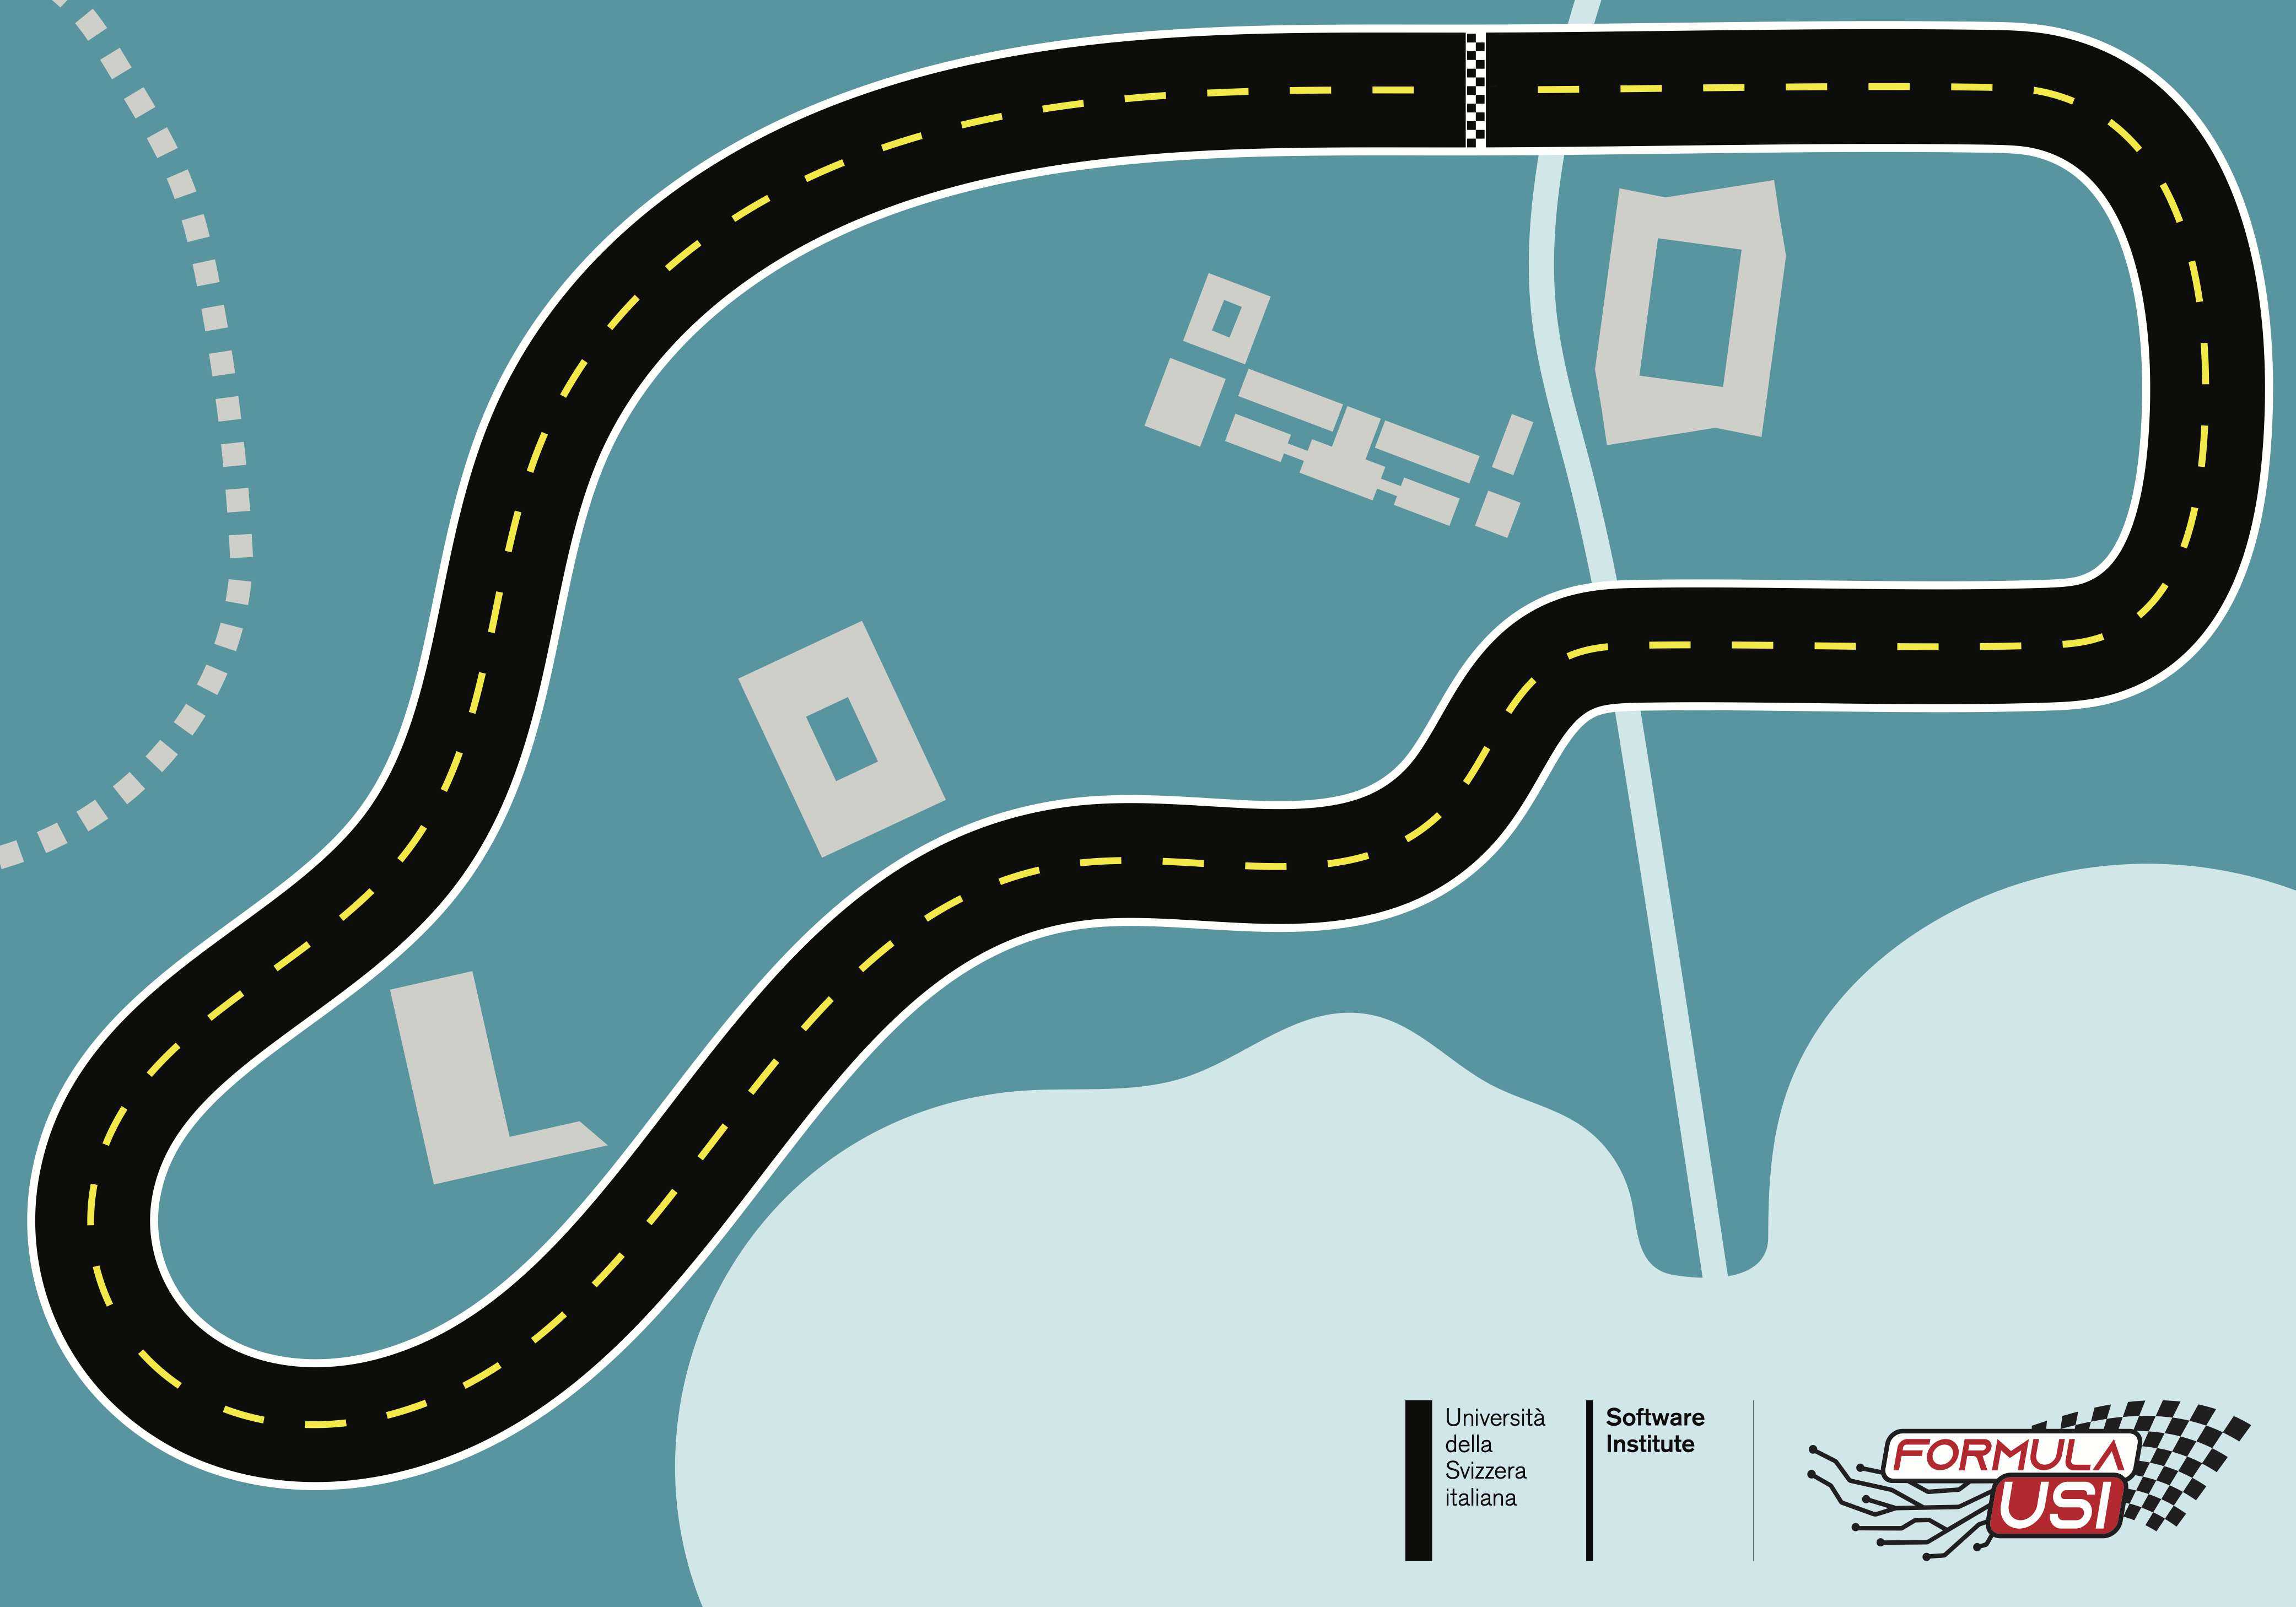
\includegraphics[width=0.85\textwidth]{setup/usi_track_real.png}
    \captionof{figure}{Real USI track TODO}
    \label{fig:usitrack}
\end{minipage}%
\begin{minipage}{.5\textwidth}
    \centering
    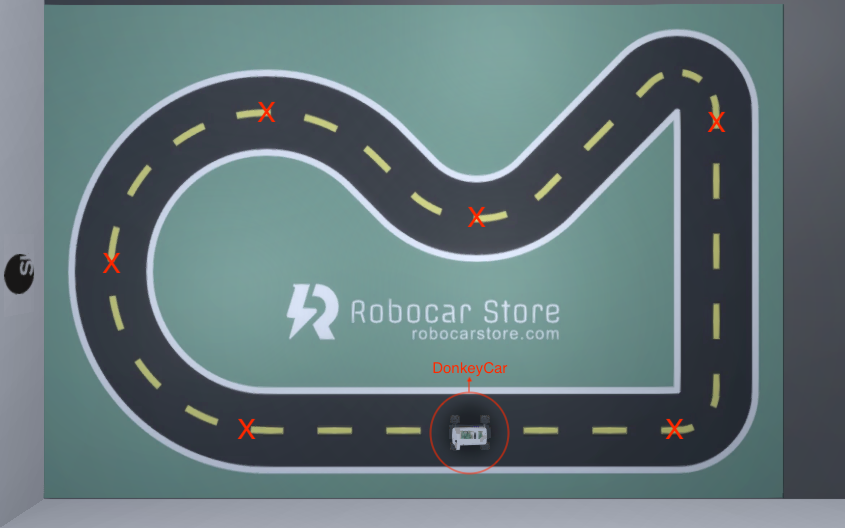
\includegraphics[width=0.95\textwidth]{setup/usi_track.png}
    \captionof{figure}{Simulated USI track}
    \label{fig:usitracksim}
\end{minipage}
\end{figure}

For our experiments in the simulated environment we used the virtual replica of such track, which was created in Unity~\footnote{https://www.unity.com} by a previous thesis in the lab. Additionally, we added a starting line in the simulated track in order to record the number of times the car completes a lap. Such information is important to understand the progress of the RL agent during training. Both tracks are single-lane, since the DonkeyCar occupies 50\% of the track when it is placed in the middle of the yellow dashed line. However, the track is an interesting testbed for RL and self-driving in general since it has a mixture of sectors that are easy to drive and curves that are challenging to take.

Regarding the Gym environment we built upon the codebase of ~\cite{learning-to-drive-in-5-minutes}. Specifically, the \textit{observation space} of both the real and simulated agent consists of RGB images of size $320 \times 240$ collected at 20\textit{Hz} (i.e. 20 frames per second). 

The \textit{action space} is composed of two continuous actions, i.e. steering and throttle, both varying in the interval $[-1, 1]$. Indeed, it is important that the action space is symmetric since most RL algorithms use a Gaussian distribution (with mean 0 and standard deviation of 1) for exploration of continuous action spaces and a non-symmetric action space would harm learning~\footnote{https://stable-baselines.readthedocs.io}. Consequently, the throttle is rescaled to take values in the interval $[0, 1]$. However, for simplicity and for speeding up learning especially in the real world, we kept the throttle constant throughout training. Furthermore, In order to obtain a smooth control of the car, the change in steering angle is \textit{constrained} by keeping an history of steering angles at previous time steps. This ensures that the difference between in steering angles in two consecutive time steps stays within a given range~\cite{learning-to-drive-in-5-minutes}.

Since we use an encoder to represent the images in a lower dimension, we used a custom Gym wrapper to convert the raw images coming from the simulator or the real world into the corresponding latent space. Moreover, we stack four consecutive frames, i.e. converted into the corresponding latent space representations, such that the agent can perceive the motion of the car by taking an action every four frames~\cite{dqn}.

Regarding the \textit{reset} of the environment we used two different modalities in simulation and in the real world. In simulation, the DonkeyCar simulator provides the \textit{cross track error} (XTE) measurement, which is defined as the distance between the center of the mass of the car and the center of the lane. Such metric varies in the interval $[-2, 2]$ when the car is \textit{fully} on-track, i.e. its center of mass is in the middle of either white lines; therefore, when the absolute value of the XTE is outside of such interval the car can be considered off-track. In particular, we used the boundary value of $3$, which corresponds to having the car with all four wheels off-track; in such case the episode terminates unsuccessfully. On the other hand, in the real world the XTE is not available. Therefore, we resort to a manual stopping strategy to terminate the episode, by remotely signaling the agent to stop controlling the car.

Finally, we established a success criterion to deem a certain episode successful. In particular, we chose to stop an episode when the number of timesteps reach the threshold level of 1000. Such threshold corresponds to approximately two laps around the track or alternatively 50 seconds given that the frame rate is 20\textit{Hz}. Indeed, the number of laps carried out by a trained RL agent depends on how \textit{smooth} is the control, since steering actually slows down the car.

%\section{The track and the environment} \label{sec:track}
%The track we used is called USI track, shown in Figure \ref{fig:usitrack}. It strongly resembles one used by \citet{DBLP:journals/corr/abs-2008-00715} in Learning to Drive. We do have a simulated version built in Unity and an actual printed track. The choice fell on this track since it is complete, it includes a straightaway, right turn, left turn, wide turn and very steep turn. Beside that, \citet{DBLP:journals/corr/abs-2008-00715} already proved that the agent can learn on this type of track and the focus of this thesis is more on replicating a real agent learning to self-drive in real world and not creating a new model with a particular feature.
%
%\begin{figure}[h]
%    \centering
%\begin{minipage}{.5\textwidth}
%    \centering
%    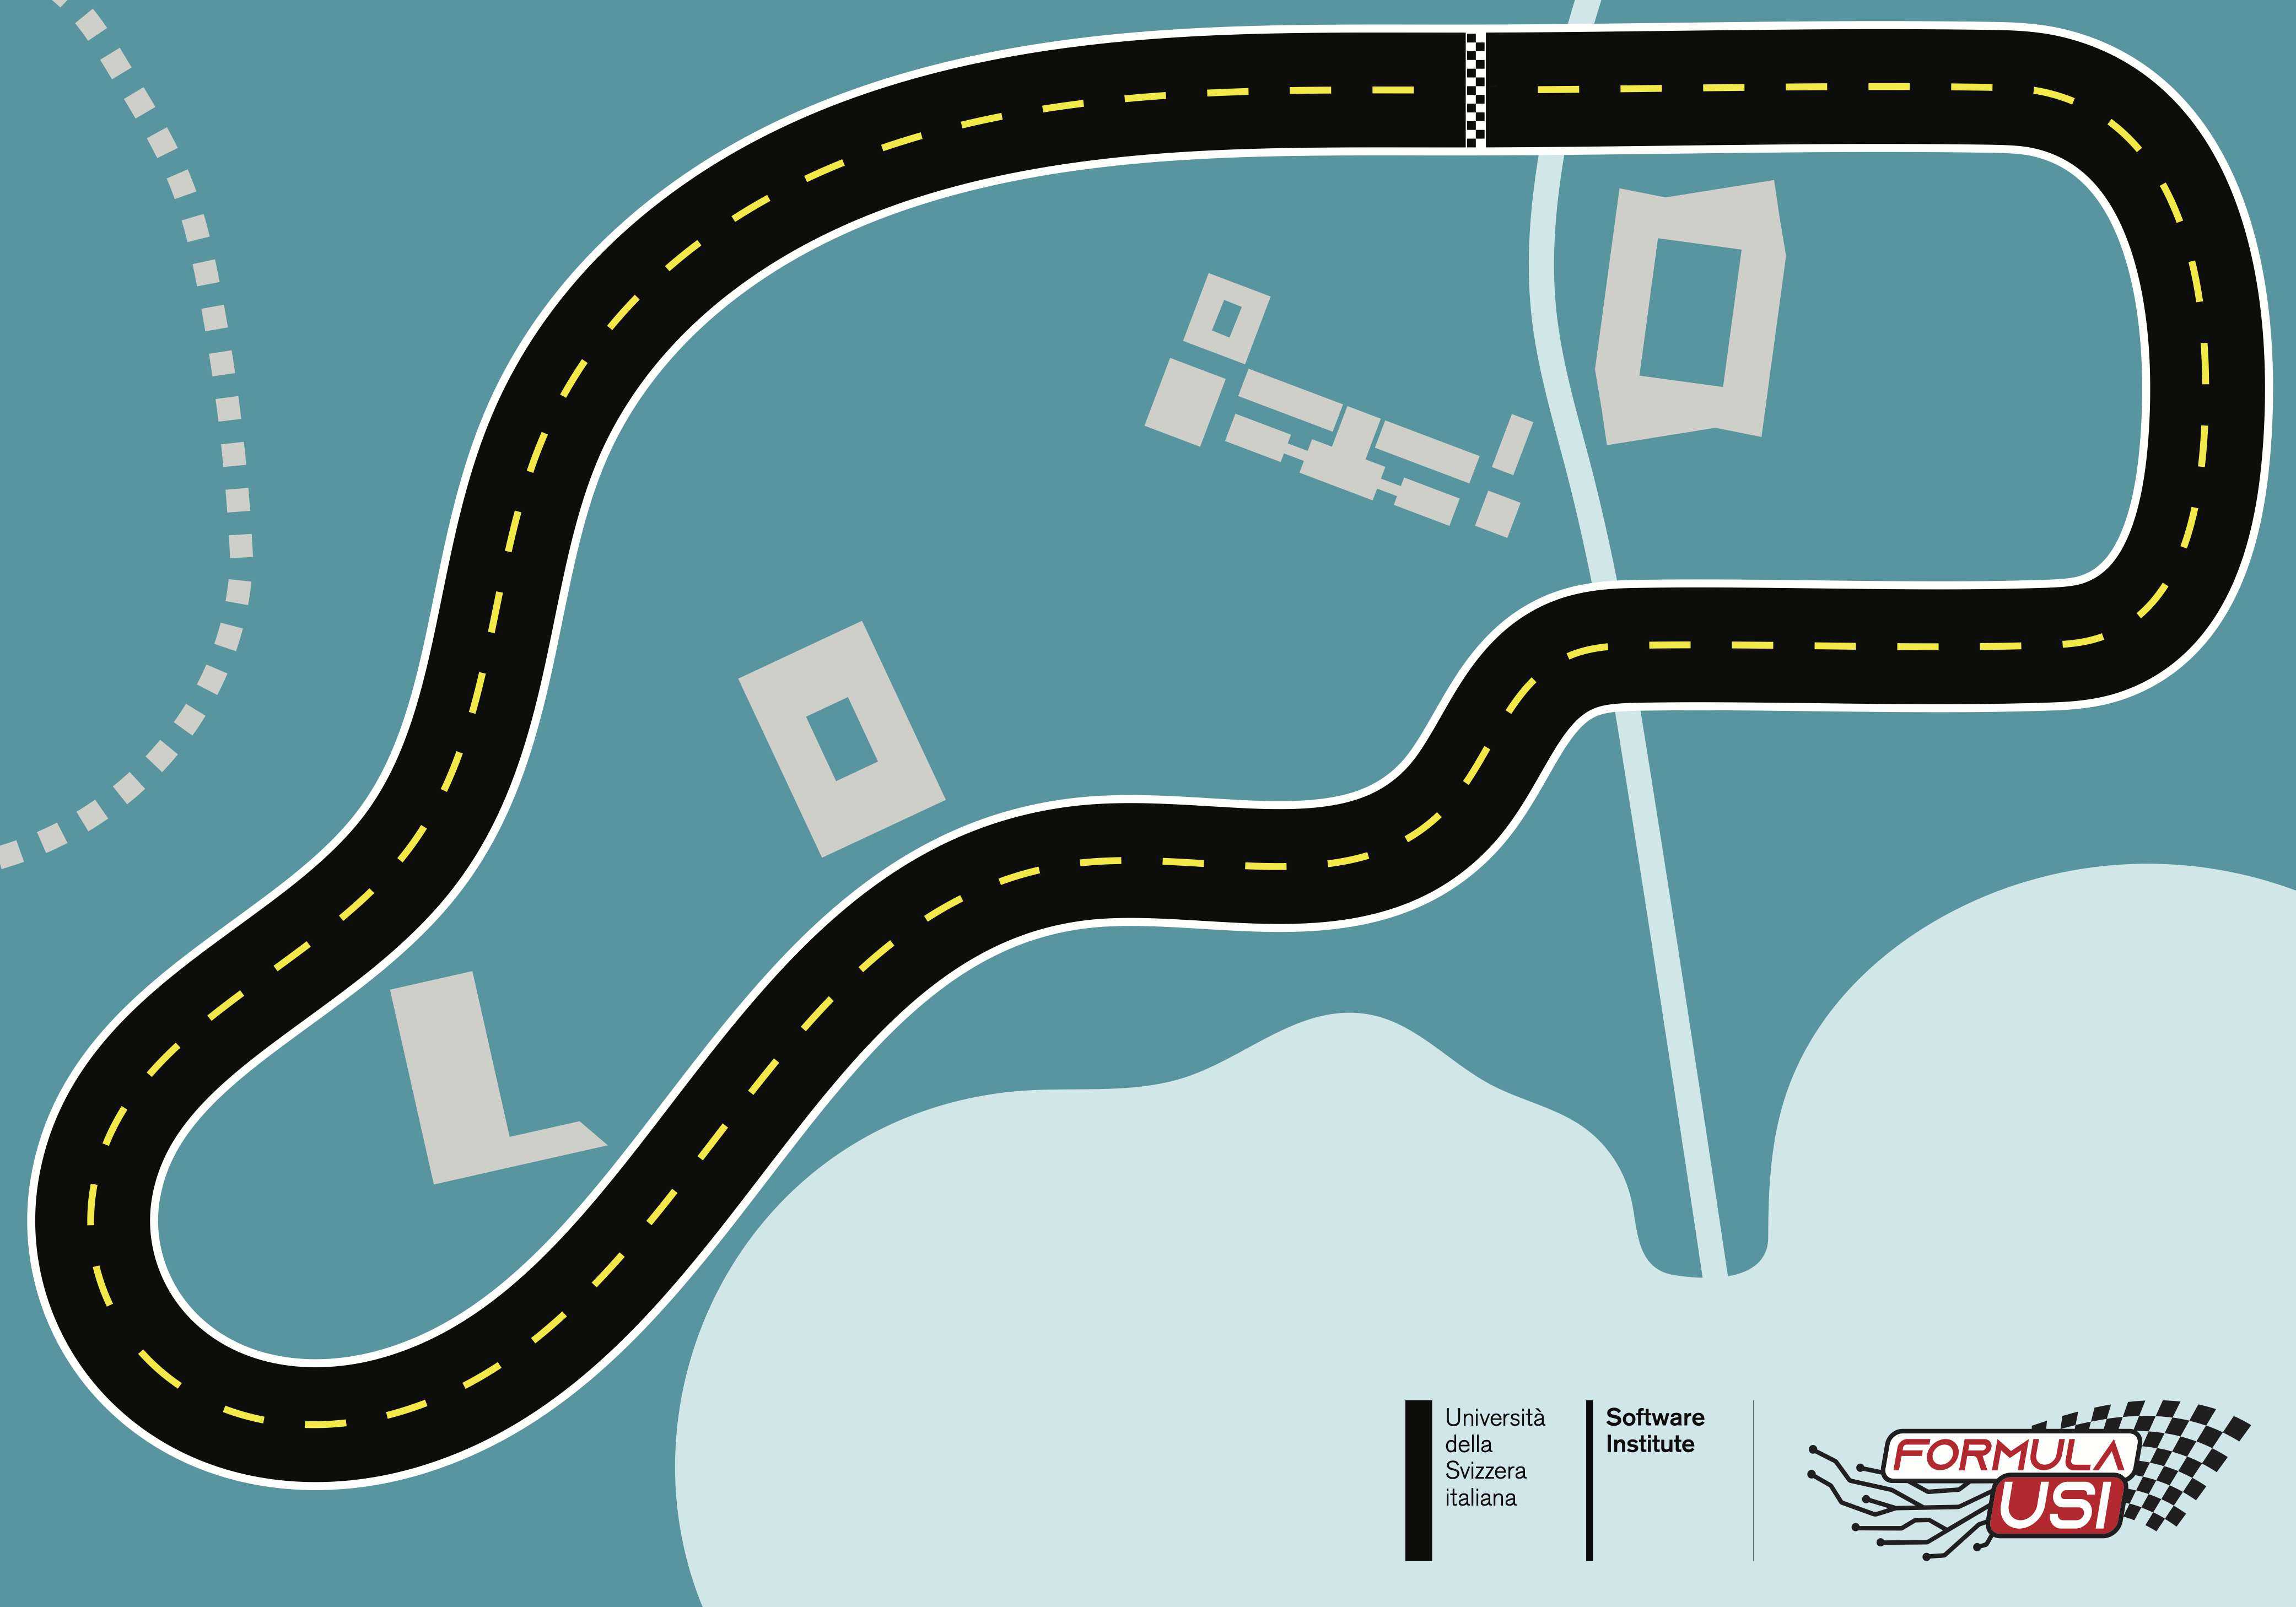
\includegraphics[width=0.85\textwidth]{setup/usi_track_real.png}
%    \captionof{figure}{Real USI track TODO}
%    \label{fig:usitrack}
%\end{minipage}%
%\begin{minipage}{.5\textwidth}
%    \centering
%    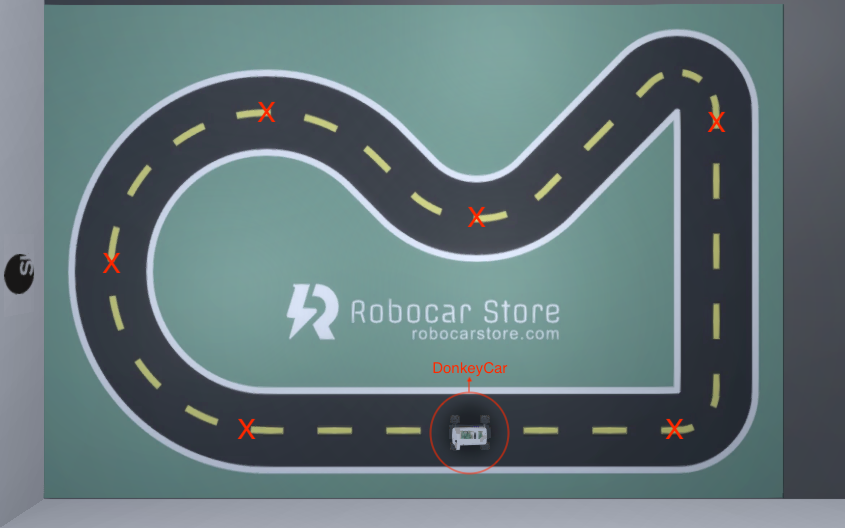
\includegraphics[width=0.95\textwidth]{setup/usi_track.png}
%    \captionof{figure}{Simulated USI track}
%    \label{fig:usitracksim}
%\end{minipage}
%\end{figure}
%
%The learning of the agent, as shown later on, is straightforward, except the very steep turn which is considerably harder than the others. This difficulty is due to the limited steering angle of the robot and in the real world the aforementioned adversity is even more marked as well see. 
%
%The default starting line in both tracks is where the Donkey is placed in Figure \ref{fig:usitracksim}. Certainly, in the real track it is an imaginary line that we use as a starting point and of course the laying of the car at each episode beginning cannot be exact but approximate. Beside that, there are a few checkpoints, approximately highlighted with a cross in Figure \ref{fig:usitracksim}, troughout the track that can be used as starting points depending on the learning strategy chosen. The simulator provides the following possibilities:
%
%\begin{itemize}
%    \item \textbf{Start:} The episode start always at the starting line.
%    \item \textbf{Checkpoint:} The episode start at the latest checkpoint reached during the previous episode.
%    \item \textbf{All:} All the checkpoints are used cyclically starting from the starting line and proceeding one by one forward for each episode.
%    \item \textbf{Random: } The starting point is chosen randomly, between the available checkpoints, at the beginning of each episode.
%\end{itemize}
%Furthermore, the simulator let us choose where a lap ends. It can end where the DonkeyCar started or at the starting line.

%TODO: AGGIUNGI referenza punti di partenza.

%\section{DonkeyCar}
%
%The real Remote Controlled DonkeyCar is essentially a standard DonkeyCar as described in Section \label{sec:donkeycar}. To recap it is a remote controlled car equipped with a microcontroller NVIDIA Netson Nano and a camera sensor. The RGB pictures are taken at a resolution of $320x240$ and at $20hz$ (20 frames per second), which means the algorithm must finish all iteration steps within $0,05$ seconds otherwise it would skip some frames and the learning or the driving may be compromised by the agent's non-responsiveness. This limitation is present only in real world since the simulator time can be slowed down to meet the needs. In our setting we have a standard 3 cell LiPO battery of 11.1V and 2200 mAh to power just the motors and the controller. During the training in the real world we often noticed a slow regression in term of speeds of the car, iteration after iteration. However, this problem can be solved by disconnecting the LiPO battery for a moment from time to time to restore full speed, which is why we suspect this problem may be caused by the battery. Furthermore, an external power bank with 10000mAh/37Wh of capacity and an output of 5V and 2.4A powers the Jetson Nano which with this capacity, is more than enough to overcome the longevity of the LiPO battery.

\section{Dataset}
In order to train the encoders for the simulated and the real world, we collected two different datasets by driving the car in the respective environment. Examples of collected images are respectively shown in Figure~\ref{fig:datasetsim} and in Figure~\ref{fig:datasetreal}.

\begin{figure}[h]
	\begin{minipage}{.33\textwidth}
		\centering
		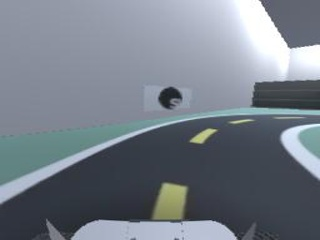
\includegraphics[width=0.95\textwidth]{setup/s1.jpg}
	\end{minipage}%
	\begin{minipage}{.33\textwidth}
		\centering
		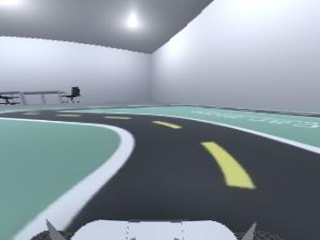
\includegraphics[width=0.95\textwidth]{setup/s2.jpg}
	\end{minipage}%
	\begin{minipage}{.33\textwidth}
		\centering
		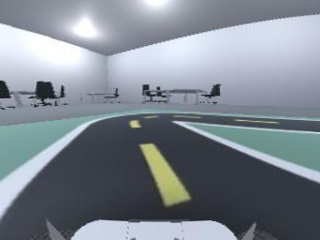
\includegraphics[width=0.95\textwidth]{setup/s3.jpg}
	\end{minipage}
	\captionof{figure}{Images extracted from the simulated dataset}
	\label{fig:datasetsim}
\end{figure}

\begin{figure}[h]
	\begin{minipage}{.33\textwidth}
		\centering
		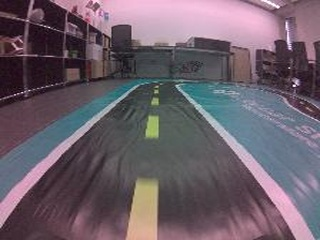
\includegraphics[width=0.95\textwidth]{setup/r1.jpg}
	\end{minipage}%
	\begin{minipage}{.33\textwidth}
		\centering
		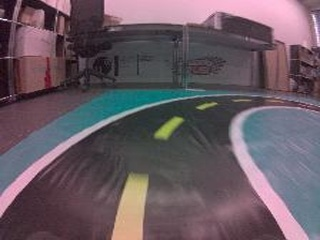
\includegraphics[width=0.95\textwidth]{setup/r2.jpg}
	\end{minipage}%
	\begin{minipage}{.33\textwidth}
		\centering
		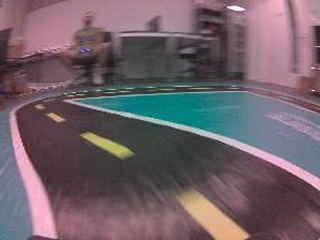
\includegraphics[width=0.95\textwidth]{setup/r3.jpg}
	\end{minipage}
	\captionof{figure}{Images extracted from the real dataset}
	\label{fig:datasetreal}
\end{figure}

In both environments we collected a dataset of $\approx$ 10\textit{k} images which correspond to $\approx$ 10 minutes of driving at $20$\textit{Hz}. We payed extra care when collecting the images in the real world by ensuring that the lighting conditions were consistent in all images; such conditions were also kept during training of the RL agent. Collecting the dataset for training the encoders does not require a good quality of driving, since labels are not recorded. However, it is important to capture all the sectors of the track such that the RL agent can extensively explore the track during training and always have a good representation of the observation it will encounter. Indeed, the pretrained encoder will not be updated during the online training of the agent.

%During the experiments resulted that a dateset of $\sim 10000$ pictures was enough to reach our goals, furthermore notice that smaller datasets may not be sufficient for the encoder to learn a good representation. To collect each of the datasets are enough $\sim10$ minutes if we run the algorithm at $20hz$ (20 frames per second) as we did. Beside that, all the pictures from the real world must be collected with a certain environmental condition that should remain consistent in time, also during the training of the agent to avoid problems. In our case, it was collected with all windows closed and the with maximum light to make it easy to be replicated. 

Before the pretraining phase of the encoder we applied a preprocessing phase of the images. In particular, we cropped the top 80 pixels from each image and resized it to $160 \times 80$. Cropping is useful to remove the part of the image that is not relevant to driving, while downscaling the image has the advantage of saving computation time when training the encoder. Figure~\ref{fig:datasetsimcropped} and Figure~\ref{fig:datasetrealcropped} show samples of cropped and resized images that are passed as input to the encoder during training. As we can see, resizing down to $160 \times 80$ does not degrade significantly the quality of the images. Moreover, the real images look like they have undergone more cropping than their simulated counterpart. The reason is that the position of the camera of the car is slightly different between simulation and real. Indeed, the \textit{simulated camera} is tilted upwards w.r.t. \textit{real camera} and this gives the impression that in the real images more pixels have been cropped.

\matteo{Le immagini in figura 4.5 non sono le corrispondenti immagini croppate e resized di figura 4.3. Lo stesso vale per le immagini reali. Uniformerei queste cose.}

%Since we want our RL agent to focus exclusively on the track we found convinient to crop the top 100 rows of each pictures to remove the background, and to reduce the complexity of our algorithm, we downscale each images from $320x140$ to $160x80$ before feeding them to the encoder. The resulting pictures are shown in Figures \ref{fig:datasetsimcropped} and \ref{fig:datasetrealcropped}. Note that during training, the training set is split in validation and training set with a ratio $20/80$ and the test set is collected apart and consist of $\sim 1000$ images for each dataset.

\begin{figure}[h]
	\begin{minipage}{.33\textwidth}
		\centering
		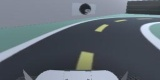
\includegraphics[width=0.95\textwidth]{setup/cs1.jpg}
	\end{minipage}%
	\begin{minipage}{.33\textwidth}
		\centering
		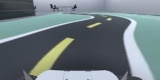
\includegraphics[width=0.95\textwidth]{setup/cs2.jpg}
	\end{minipage}%
	\begin{minipage}{.33\textwidth}
		\centering
		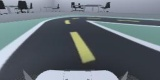
\includegraphics[width=0.95\textwidth]{setup/cs3.jpg}
	\end{minipage}
	\captionof{figure}{Examples of cropped simulated images}
	\label{fig:datasetsimcropped}
\end{figure}

\begin{figure}[h]
	\begin{minipage}{.33\textwidth}
		\centering
		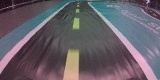
\includegraphics[width=0.95\textwidth]{setup/cr1.jpg}
	\end{minipage}%
	\begin{minipage}{.33\textwidth}
		\centering
		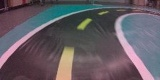
\includegraphics[width=0.95\textwidth]{setup/cr2.jpg}
	\end{minipage}%
	\begin{minipage}{.33\textwidth}
		\centering
		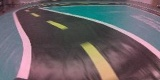
\includegraphics[width=0.95\textwidth]{setup/cr3.jpg}
	\end{minipage}
	\captionof{figure}{Examples of cropped real images}
	\label{fig:datasetrealcropped}
\end{figure}

Finally such images collected in the simulator and in the real world are also useful for training the CycleGAN architecture~\cite{CycleGAN2017}. In order to save computation time the dataset we provided to the CycleGAN training process is smaller, i.e. $\approx$ 5\textit{k} images for each domain, i.e. simulated and real, since previous work shows that such size is adequate to represent the track we are considering~\cite{stocco-mind}.

%Finally, for the cyclegan, the dataset can be even smaller $\sim 5000$ pictures for both real and simulation. No crop is applied and a resize to $256x256$ pixels is done to match the network size provided by \citet{CycleGAN2017}. And the test sets match the ones used for the encoders. After applying the cyclegan in our experiments, the pictures are reshaped and cropped to match the need of the autoencoder.

\section{Training}

To train the RL agent we adopted the SAC algorithm due to its sample efficiency and the ability to reuse the collected experience~\cite{art:sac}. Such abilities are paramount when training an agent in the real world. We used the hyperparameters provided by \cite{learning-to-drive-in-5-minutes} for the task of driving. In particular, we chose a replay buffer of size $300$\textit{k} (i.e. the number of transitions that can be stored) and a multilayer perceptron with two layers of 64 units each both for the actor and the critic. Moreover, training is carried out at the end of each episode for 64 gradient steps. \matteo{Mi sembra che nel reale la policy sia piu' grande, forse sono 4 layer da 64 unita'. Giorgio check.} Thanks to the dimensionality reduction step, the transitions in the replay buffer contain latent vectors rather than entire images; as a consequence training is relatively fast and it can be carried out in machine without GPU. 

%\subsection{Simulation}\label{subsec:sim}
In simulation, the training is performed using a client-server architecture where both client and server run on the same machine. The server, i.e. the Donkey simulator, provides the frames captured by the simulated camera at each timestep together with the \textit{telemetry} of the car, i.e. its position, velocity and XTE. The client, i.e. the learning component, receives the frames and the telemetry and it is tasked to make a control decision, i.e. it has to return to the server the action to undertake on the car. Once the server receives the action, the simulator applies it on the car and the cycle continues. The decision to start or stop an episode is delegated to the client, which according to the telemetry received by the simulator at each step, decides when to reset the environment. When an episode terminates, the training procedure starts. Afterwards the simulation is stopped for the entire duration of training and it is resumed as soon as the training finishes.

Also In the real environment we used a client-server architecture for training. However, client and server run on different machines. This is because the Donkey microcontroller has limited computation capabilities and, most importantly, a limited battery. Indeed, carrying out the RL agent training on the Donkey would quickly deplete the battery and slow down training due to frequent battery recharge and replacement. Moreover, having two dedicated machines also allows a human operator to remotely stop an episode, appropriately reset the car to its initial position and remotely restart it.

In particular, we used the MQ Telemetry Transport (MQTT) messaging protocol, which is one of the most used in the internet of things domain. The protocol defines all the rules that determine how devices exchange messages over the internet, i.b. by writing (publish) and reading (subscribe) data. The sender (publisher) and the receiver (subscriber) communicate on message channels called \textit{topics} and are decoupled from each other. The protocol also involves the presence of a \textit{broker} that has access to the incoming messages and distributes them correctly to the subscribers of a certain topic. Specifically, we used the \textit{HiveMQ} broker which allows the connection of up to 100 clients free of charge. The topics defined to manage the communication between the DonkeyCar and the client machine are as follows:

\begin{itemize}
    \item \textbf{Stop car:}. (Client - Publisher, Donkey - Subscriber). When the client machine publishes a message on this topic the RL agent on the Donkey stops controlling the car, i.e. the episode must terminate. Practically the human operator presses the space bar on the keyboard which triggers the signal;
    \item \textbf{Replay buffer:} (Donkey - Publisher, Client - Subscriber). Once an episode terminates, the Donkey publishes on this topic all the transitions collected during the episode. The client machine receives such transitions and stores them in the replay buffer which is used to train the policy. The transitions only contain the latent space representations of the captured images in the real world; indeed, the encoder runs on the Donkey and transforms each frame into its corresponding latent space representation in order to be processed by the policy. This way the transitions exchange is quicker than sending raw images;
    \item \textbf{Replay buffer received:} (Client - Publisher, Donkey - Subscriber). The client uses this topic to acknowledge the Donkey that it has received the transitions collected during the just terminated episode. \matteo{perche' e' utile questo topic? Che cosa fa la Donkey una volta ricevuto questo messaggio?}
    \item \textbf{Parameters:} (Client - Publisher, Donkey - Subscriber). The client has a copy of the parameters of the policy used by the Donkey. Once the client receives the transitions the training starts. During training the human operator can retrieve the car and position it back on track. Once the training is complete, the client machine publishes the updated policy parameters and the Donkey updates its copy of the policy parameters;
    \item \textbf{Start episode:} (Client - Publisher, Donkey - Subscriber). The client uses this topic to acknowledge the Donkey that a new episode must start. Practically the human operator presses the enter key on the keyboard which triggers the signal;
\end{itemize}

%\section{Communication - MQTT}
%
%As described in Section \ref{subsec:real}, when training in real world, the host machine and the DonkeyCar must communicate wirelessly multiple times during the training. MQ Telemetry Transport (MQTT) is the most used messaging protocol for the Internet of Things (IoT). It includes all the rules that define how devices can write (publish) and read (subscribe) data over the internet. The sender (Publisher) and the receiver (Subscriber) communicate via topic and are decoupled from each other. The connection between them is handled by an MQTT broker that filters all incoming messages and distributes them correctly to the Subscribers of the topic. In pratice any device can publish a message on a topic, then the broker take care of dispatching it to subscribers of that topic. In particular we used the HiveMQ broker that allows the connection of up to 100 clients with no cost. The topics defined to manage the communication between the host machine and the DonkeyCar are:
%
%\begin{itemize}
%    \item \textbf{Stop car:} The host machine writes a signal on this topic, that is constantly monitorated by the DonkeyCar, to inform that the episode must terminate.
%    \item \textbf{Replay buffer:} Once the episode terminate, all the collected information by the DonkeyCar are sent to the host machine through this topic.
%    \item \textbf{Replay buffer received:} The host machine uses this topic to acknowledge DonkeyCar that it has received the buffer.
%    \item \textbf{Parameters:} Once the training is complete, the host machine sent the updated neural network parameters through this topic.
%    \item \textbf{Start episode:} The host machine uses this topic to acknowledge DonkeyCar that a new episode can start.
%    \item \textbf{Speed modifier:} This topic can be used by the host machine to inform the DonkeyCar that it must change its throttle by the sent value that can be either positive or negative.
%\end{itemize}


%\section{Training modality}
%
%\subsection{Simulation}\label{subsec:sim}
%In simulation, the training of the agent is straightforward since all the operation are done on the host machine, moreover it is not required a GPU machine to accomplish all the steps in time, at least until the cyclegan is introduced. Even though an on-policy RL algorithm could be implemented, an off-policy algorithm is chosen since in real world, in our setting, the on-policy method is not replicable given the limited computational power of the microcontroller. Beside that, we want to compare the same type of algorithm in the two type of environments. In pratice, a pretrained AE/VAE provides a representation of the state in the form of a latent vector, the agent drives with a policy kept constant during the episode and all the frames and actions are collected into a buffer. When the simulator reports that the car has crashed or went out of track more than a predefined distance, the episode terminates. The episode ends also when the car has reached the starting point or, in our setup, it reaches 1000 steps. Finally, at the end of the episode, a policy is trained using the collected buffer and the new parameters are used to update the driving policy.
%
%\subsection{Real world} \label{subsec:real}
%Since the microcontroller equipped by the DonkeyCar is a low capability calculator, a few precautions need to be taken in order to to train the agent. Firstly, as mentioned above, an off-policy method like SAC allows to relocate the actual training, and consequently the very expensive gradient back-propagation, to another machine with more resources. Secondly, the use of representation learning (AE/VAE) allows to reduce significantly the size of the RL neural networks and moreover the pre-training of the encoder can be done in advance on the host machine speeding up the process. In practice the functioning is similar to the one seen in previous Section \ref{subsec:sim}. The microcontroller operates the driving policy, collect the image, forward it through the AE/VAE, then the agent chose an action based on that representation. This process is repated until a human supervisor ends the episode for the car gone off the track. The episode also terminates when the DonkeyCar reaches, in our setup, 1000 steps. Hereafter, all the steps information, like latents vectors, actions and rewards are collected into a buffer up to a predefined size and are sent through the network to the host calculator that actually train the policy at the end of the episode. After the training, the new parameters are sent back to the DonkeyCar and the process is repeated until convergence.
%
%\section{Communication - MQTT}
%
%As described in Section \ref{subsec:real}, when training in real world, the host machine and the DonkeyCar must communicate wirelessly multiple times during the training. MQ Telemetry Transport (MQTT) is the most used messaging protocol for the Internet of Things (IoT). It includes all the rules that define how devices can write (publish) and read (subscribe) data over the internet. The sender (Publisher) and the receiver (Subscriber) communicate via topic and are decoupled from each other. The connection between them is handled by an MQTT broker that filters all incoming messages and distributes them correctly to the Subscribers of the topic. In pratice any device can publish a message on a topic, then the broker take care of dispatching it to subscribers of that topic. In particular we used the HiveMQ broker that allows the connection of up to 100 clients with no cost. The topics defined to manage the communication between the host machine and the DonkeyCar are:
%
%\begin{itemize}
%    \item \textbf{Stop car:} The host machine writes a signal on this topic, that is constantly monitorated by the DonkeyCar, to inform that the episode must terminate.
%    \item \textbf{Replay buffer:} Once the episode terminate, all the collected information by the DonkeyCar are sent to the host machine through this topic.
%    \item \textbf{Replay buffer received:} The host machine uses this topic to acknowledge DonkeyCar that it has received the buffer.
%    \item \textbf{Parameters:} Once the training is complete, the host machine sent the updated neural network parameters through this topic.
%    \item \textbf{Start episode:} The host machine uses this topic to acknowledge DonkeyCar that a new episode can start.
%    \item \textbf{Speed modifier:} This topic can be used by the host machine to inform the DonkeyCar that it must change its throttle by the sent value that can be either positive or negative.
%\end{itemize}
%
%Notice that this protocol is not complety reliable so some precautions and check must be done when implenting it, especially in real-time system where some actions cannot be delayed.